This section provides a brief overview of background information relevant to the thesis. First, a concise review of cloud computing is presented. Then, the concept of containerization is discussed and Kubernetes is introduced as a possible container orchestration framework. An overview of relevant Kubernetes terminology and mechanisms is provided. Finally, the section elaborates on both general and Kubernetes-specific autoscalers.


\subsection{Cloud Computing}
Companies eliminate the cost of acquiring and managing hardware by moving their services to the cloud. In cloud computing, access to a configurable resource pool is provided over a network\citep{NIST-Could-Def}. Three main models of cloud computing are distinguished based on the type of resources provided\citep{NIST-Could-Def}: 
\begin{itemize}
    \item \textit{Infrastructure as a Service (IaaS)} offers fundamental computational resources like processing power and storage to customers. These resources could be offered in the form of virtual machines (VM's). Examples are Amazon's Elastic Compute Cloud (EC2) and Microsoft Azure.
    
    \item \textit{Platform as a Service (PaaS)} provides customers with a platform on which they can deploy their own applications without having to manage the underlying hardware. This enables developers to focus entirely on the development of applications. Examples are Google App Engine and OpenShift. 
    
    \item In \textit{Software as a Service (SaaS)}, the provider offers a specific application to its customers. Instead of users having to run the application locally, it is run and managed by the provider. Examples are Salesforce and Google Apps. 
\end{itemize}

\subsubsection{Service Level Agreements}
Services delivered by cloud providers are usually documented in a service level agreement (SLA). An SLA includes, among others, a description of the provided services and the expected quality of the services \citep{SLA2}. The quality of service (QoS) can in turn be documented in a series of service level objectives (SLOs). An SLO defines one measurable characteristic of an SLA. It usually includes an achievement level, a target measurement, a measurement period and a manner to measure the metrics. An example would be ``Measured over a one year period, the application should be available 99.5\% of the time, as measured by the heartbeat system'' \citep{SLO}\citep{SLO2}.

\subsection{Containerization}
Deploying an application on the cloud requires a way of executing it independently of the underlying hardware. Furthermore, applications should not be affected by any other applications running on the same hardware. Virtualization isolates an application and its dependencies into a self-contained unit that can be run anywhere\citep{Virtualization}.
Virtualization is implemented either at hardware level or at operating system level. \\

With hardware level virtualization, a virtual machine (VM) combines the applications to be run, their dependencies and an operating system (OS). VMs are run on top of a hypervisor (also known as a virtual machine monitor), which is a process that creates, runs and manages VMs. The hypervisor, in turn, runs on the host infrastructure. With operating system virtualization, on the other hand, a container bundles the application and its dependencies, and is run on top of a container engine (Docker, for example). Figure \ref{fig:container_vs_vm} shows both virtualization mechanics. Because containers are more lightweight, they have grown in popularity in the last years\citep{Container}. \\

\begin{figure}[h]
\begin{center}
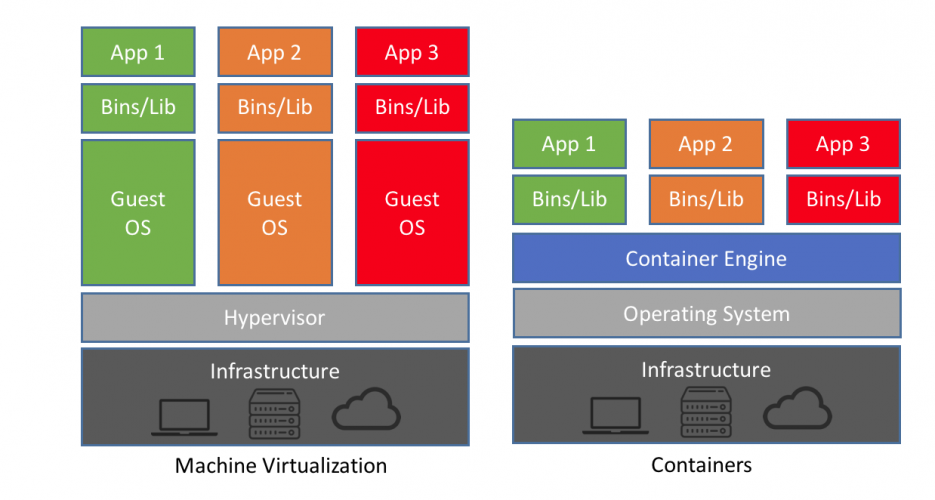
\includegraphics[width=0.9 \textwidth]{Images/VM_vs_container.png}
\end{center}
\caption{Virtual machine vs container \citep{Container-vs-vm}}
\label{fig:container_vs_vm}
\end{figure}

\newpage

Linux containers (LXCs) provide several features to manage applications running in them, the most important ones being control groups (cgroups) and namespaces. Cgroups provide a unified interface to manage processes and their resources, including resource monitoring and limiting, prioritization and control\citep{Cgroup}. Namespaces are used to isolate a processes' resources. This makes it appear to the processes within the namespace that they have access to their own isolated instance of a global resource\citep{Namespace}.

\subsubsection{Docker}
Docker is a container engine designed to manage Linux containers. It offers functionalities to develop, ship and run applications through container-based virtualization\citep{Docker}. Containers in Docker are created through Docker images, which are read-only templates with instructions for creating the Docker container \citep{Docker-image}. How to build a Docker image is, in turn, documented in a Dockerfile. Figure \ref{fig:dockerfile} shows an example Dockerfile. Docker is, however, limited to the management of containers on a single machine.

\begin{figure}[h]
\begin{center}
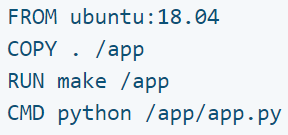
\includegraphics[width=0.35 \textwidth]{Images/Dockerfile.PNG}
\end{center}
\captionsetup{justification=centering}
\caption{Dockerfile example. FROM creates the starting layer, COPY adds files, RUN executes a command and CMD provides the default command and arguments for the container\citep{Dockerfile}.}
\label{fig:dockerfile}
\end{figure}

\subsection{Kubernetes}
When deploying applications in a distributed context, managing them becomes a challenge. Container orchestration engines like Kubernetes provide multiple features to manage distributed systems effectively. Kubernetes is an open source container orchestration engine providing basic mechanisms for the deployment, maintenance, and scaling of applications \citep{kubernetes_github}.

\subsubsection{Terminology}

\paragraph{Pod} A pod is the smallest deployable unit in Kubernetes, as mentioned in the introduction. It encapsulates one or more containers, storage resources and a unique network IP. Each pod is meant to run a single instance of a given application. Figure \ref{fig:pod} shows an example definition of a pod definition \citep{Kubernetes-Pod}.

\begin{figure}[h]
\begin{center}
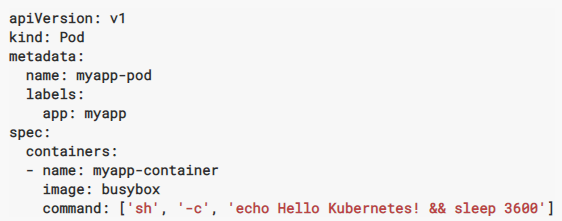
\includegraphics[width=0.90 \textwidth]{Images/Pod_example.PNG}
\end{center}
\captionsetup{justification=centering}
\caption{Pod definition example. The pod contains one container, called \textit{`myapp-container'}, which is based on the \textit{`busybox'} Docker image \citep{Kubernetes-Pod}.}
\label{fig:pod}
\end{figure}

\paragraph{ReplicaSet}
If multiple replicas of identical pods ar required to run at all times for, for example, availability purposes, a ReplicaSet can be defined. A ReplicaSet's definition includes the specifications of the pod and the amount of replicas which should be maintained\citep{Kubernetes-ReplicaSet}.

\paragraph{Deployment}
Pods and ReplicaSets may need to be updated during operations. A Deployment describes the desired state of either a pod or a ReplicaSet. Typical use cases of Deployments are:
\begin{itemize}
    \item Rolling out a ReplicaSet by creating a Deployment;
    \item Declaring the new state of a pod by updating a Deployment;
    \item Rolling back to an earlier Deployment;
    \item Scaling up or down the amount of replicas;
    \item Pausing and resuming a Deployment to apply fixes;
    \item Checking the status of a Deployment; and
    \item Removing unused ReplicaSets \citep{Kubernetes-Deployment}.
\end{itemize}

\paragraph{StatefulSet}
StatefulSets are similar to Deployments but provide additional guarantees about the ordering and uniqueness of the pods. They are typically used when any of the following features is desired:
\begin{itemize}
    \item Stable and unique network identifiers;
    \item Stable and persistent storage;
    \item Ordered and graceful deployment and scaling; and
    \item Ordered and automated rolling updates \cite{Kubernetes-StatefulSet}.
\end{itemize}

\paragraph{Service}
Pods, by themselves, terminate without healing if anything goes wrong. ReplicaSets maintain a stable amount of identical pods, but the pods may be killed and recreated at any time. Since each pod gets its own IP address, the IP adress at which an application can be reached is subject to change. Services solve this problem by defining a set of logical pods and a policy by which to access them. Other applications then communicate with the application by addressing its Service \citep{Kubernetes-Service}.

\paragraph{Requests and limits}
Users may specify the requests and limits of a pod. A pod is always guaranteed to get its requested amount of resources, and may use up to its specified limit when there are free resources in the node. The sum of the requests of all the pods running in a node should be less than or equal to the total amount of available resources of that node. The sum of limits, however, can be higher than the available resources of the node, allowing for oversubscription of that node. At the time of writing, Kubernetes only supports requests and limits for CPU and memory \citep{requestlimit}.

\paragraph{Quality of Service classes}
Based on the requests and limits of a pod, Kubernetes automatically assigns it a Quality of Service (QoS) class. A pod is assigned the `Guaranteed' QoS class if every container in the pod has specified limits and optionally requests, and if the requests are all equal to the limits. A pod is assigned the `Burstable' QoS class if requests and optionally limits are set for any container in the pod, and they are not equal. If no requests or limits are set for any container in the pod, the pod gets the `Best Effort' QoS class \citep{QoS}.

\subsubsection{Kubernetes out-of-resource handling}\label{background:oversubscription}

In an oversubscribed node, Kubernetes divides the free resources among the pods based on their requests, limits and QoS classes. When the workload grows, pods may need to contend for the free resources in the node. Depending on the type of the bottleneck resource, one of two things can happen. If the resource is compressible (able to be throttled), CPU for example, then the pod with the lowest request gets throttled. This allows the pod with the higher request to use a bigger part of the free resources. If the bottleneck resource is not compressible, like memory, the pod with the lowest QoS class gets evicted instead. \\

Kubernetes throttles pods as follows. It converts the requested CPU to its core value (so 500 millicores = 0.5 CPU) and multiplies it by 1024. A pod's \textit{cpu-shares} value is then set to the greater of this calculated number or 2 \citep{Kubernetes-cpu-shares}. When there are sufficient CPU cycles available for all containers, each container may use as much of them as needed, up to their specified limits. When CPU becomes limited, however, it is divided according to the relative weight of the \textit{cpu-shares} values. So, for example, if two containers have CPU requests of respectively \textit{1000m} and \textit{500m}, then, when CPU becomes limited, the first container receives 66\% of the CPU cycles, while the second one only receives 33\%\citep{Docker-cpu-shares}.\\

\subsection{Autoscaling}
The goal of an autoscaler is to automatically adjust an application's resources based on its needs at any given time. Three main characteristics distinguish autoscalers. 
The first one is when it decides to scale, also referred to as the scaling model. This can be either reactively or proactively. Reactive approaches, as the name suggests, react to changes without anticipating them, while proactive approaches use forecasting techniques to determine when an application should be scaled. Some autoscalers use a combination of proactive and reactive approaches. 
A second characteristic is how the actual scaling is performed, also known as the scaling method. This can be through vertical scaling, horizontal scaling or a combination of both. Vertical scaling entails increasing the capacity of existing entities in the system. For example, if an application is deployed using virtual machines, the amount of memory to which a virtual machine has access could be increased or decreased. Horizontal scaling is achieved by adding or removing entities to the system, for example by adding or removing virtual machines. The third characteristic is which metrics are considered when making scaling decisions, for example CPU or memory usage \citep{CoutinhoEmanuel2015Eicc}. 

\subsubsection{Autoscaling in Kubernetes}
As mentioned before, Kubernetes offers a default horizontal autoscaler called the Horizontal Pod Autoscaler (HPA)\citep{HPA}. It is a purely reactive autoscaler which only bases its scaling decisions on CPU utilization by default. The HPA can be extended to support other scaling metrics. It makes scaling decisions using threshold-based policies. With such policies, certain thresholds are set for resource utilization or SLA violations and when they are crossed, the application should be scaled. Care has to be taken when implementing these thresholds, as oscillating metrics could lead to unnecessary scalings. An example of an unsafe or incomplete rule set would be ``if memory usage is greater than 80\%, a replica should be added'' paired with ``if memory usage is less than 80\%, a replica should be removed''. When the memory usage oscillates around 80\%, the autoscaler may decide constantly change the amount of replicas. This is sometimes referred to as thrashing. A better rule would be ``if memory usage is greater than 80\% for 5 minutes, the a replica should be added'', and vice versa. The Kubernetes HPA offers such thrashing prevention by including a certain scaling delay by default.\\

The Kubernetes community is also working on a Vertical Pod Autoscaler (VPA)\citep{VPA}. A drawback of this autoscaler is that it needs to restart a pod when scaling it. Moreover, this autoscaler is not included by default.

